\documentclass[addpoints]{exam}
\usepackage{url}
\usepackage{amsmath,amsthm,amssymb}
\usepackage{graphicx}
\usepackage{tikz}
\usepackage{cancel}
\usepackage{float}
\usepackage{caption}
\usepackage{soul}
\usepackage{units}
\usepackage{algorithmic}
\usetikzlibrary{positioning}
\def\checkmark{\tikz\fill[scale=0.4](0,.35) -- (.25,0) -- (1,.7) -- (.25,.15) -- cycle;} 

\newcommand{\Exval}[1]{\left< #1\right>}
\newcommand{\ExvalDef}[1]{\sum_{i=0}^{\infty} #1P\left( #1\right)}
\newcommand{\Var}[1]{\sigma^{2}\left( #1\right)}
\newcommand{\VarDef}[1]{\left< #1^{2}\right> - \left< #1\right>^{2}}
\newcommand{\BigO}[1]{\mathcal{O}\left( #1\right)}
\newcommand{\BigT}[1]{\Theta\left( #1\right)}
\newcommand{\BigOmega}[1]{\Omega\left( #1\right)}
\newcommand{\T}[1]{T\left( #1\right)}
\renewcommand{\P}[1]{\left( #1\right)}
\newcommand{\floor}[1]{\lfloor #1\rfloor}
\newcommand{\ceil}[1]{\lceil #1\rceil}
\newcommand{\abs}[1]{\left| #1\right|}
\newcommand{\Lim}[1]{\raisebox{0.5ex}{\scalebox{0.8}{$\displaystyle \lim_{#1}\;$}}}


\newtheorem{lemma}{Lemma}[section]
\newcommand{\var}{\text{Var}}
\author{Christopher Mertin\\{\small (Worked with Johnny Walker, Jack Daniels, and Jim Bean)}}
\title{CS 6150: Homework 2}
\date{Due Date: October 1, 2015}
\begin{document}
\maketitle
\begin{center}
\fbox{\fbox{\parbox{5.5in}{\centering
This assignment has \numquestions\ questions, for a total of \numpoints\
points. 
Unless otherwise specified, complete and reasoned arguments will be expected for all answers. }}}
\end{center}

\qformat{Question \thequestion: \thequestiontitle\dotfill \textbf{[\totalpoints]}}
\pointname{}
\bonuspointname{}
\pointformat{[\bfseries\thepoints]}

\printanswers

\begin{center}
  \gradetable
\end{center}
  \ \\\ \\\ \\{\bf \large Equation Definitions}
  \begin{align*}
    \intertext{\underline{Expectation Value:}}
    \Exval{X} &= \ExvalDef{x}\\
    \intertext{\underline{Variance:}}
    \Var{X} &= \VarDef{X}\\
    \intertext{\underline{Standard Deviation:}}
    \sigma (X) &= \sqrt{\Var{X}}
  \end{align*}
\newpage

Here are the three increasingly-strong inequalities we use to analyze the tail
of a distribution. 

\begin{lemma}[Markov]
  Let $X$ be a random variable taking nonnegative values. Then for any $a > 0$,
\[ \Pr(X \ge a) \le \frac{\Exval{X}}{a} \]
\end{lemma}

\begin{lemma}[Chebyshev]
  Let $X$ be a random variable with bounded variance. Then 
\[ \Pr(|X - \Exval{X}| \ge a) \le \frac{\Var{X}}{a^2} \]
\end{lemma}
\begin{lemma}[Chernoff]
  Let $X_1, \ldots, X_n$ be independent random variables taking the values $0, 1$ with $E[X_i] =
  \Pr(X_i = 1) = p_i$. Let $\mu = \sum_i p_i$. Then for any $\delta > 0$, 
\[ \Pr(X \ge \mu(1+\delta)) \le \exp\left( - \frac{\mu \delta^2}{3}\right) \]
\[ \Pr(X \le \mu(1-\delta)) \le \exp\left( - \frac{\mu \delta^2}{2}\right) \]
\end{lemma}
\begin{questions}
\titledquestion{Tail Bounds I}
\begin{parts}
\part[5] The Markov inequality yields an \emph{upper} bound on the probability
  of going far away from the mean. It is reasonable to ask whether we can do
  better. Show that you can't, by constructing some nonnegative random variable
  $X$ and a value $a > 0$ such that 
\[ \Pr(X \ge a) = \frac{\Exval{X}}{a} \]

\begin{solution}
\begin{align}
\intertext{The definition of the expected value is as follows:}
\Exval{X} &= \ExvalDef{X} = \sum_{i=0}^{\infty}P(X\geq i)\\
\intertext{Since the range of the set is finite and of size $a$, and since $a > 0$}
\Exval{X} &\geq \sum_{i=0}^{a-1}P(X\geq i)\\
\intertext{And since $i < a$, we can use that in the probability}
\Exval{X} &= a\cdot P(X\geq a)\\
\frac{\Exval{X}}{a} &= P(X\geq a)
\end{align}
\end{solution}
\newpage
  \part[5] Suppose we roll a fair die $100$ times. Determine the probability
  that the sum of the rolls is at least  $400$ (using Markov's inequality) and
  the probability it is
  not in the range $[301,399]$ (using Chebyshev's inequality).

  \begin{solution}
  \begin{align}
    \intertext{Expectation value of a dice roll is defined as}
    \Exval{X} &= \ExvalDef{X} = \sum_{i=1}^{6}i\cdot P(i) = \frac{1}{6}(1+2+\cdots +6) = \frac{21}{6} = 3.5\\
    \intertext{That means that the expected value of 100 rolls is}
    \Exval{X}_{100} &= 350\\
    \intertext{Using the Markov Method to calculate the probability of the sum being more than 400}
    P(X\geq 400) &= \frac{350}{400}
    \intertext{Now for in the probability {\bf NOT} in the range of $[301,399]$. The first the squared expectation value is needed for a single dice roll}
    \Exval{X^{2}} &= \frac{1}{6}\sum_{i=1}^{6}i^{2}=\frac{91}{6}\\
    \intertext{Where the variance can also be calculated from this}
    \Var{X} &= \frac{91}{6} - 3.5^{2} = 2.917\\
    \Var{X}_{100} &= 291.7\\
    \intertext{And the use of the Chebyshev Inequality leads to using $a = 50$ since the range that we are wanting is 100 $[301,399]$ which is 50 in each direction (since the probability is denoted in each direction).}
    P\P{\abs{X-\Exval{X}}\geq 50} &= \frac{291.7}{50^{2}}\approx 0.1167
  \end{align}
  \end{solution}

  \part[5] Suppose we're given an algorithm that takes as input a string of $n$
  bits. We are told that the expected running time is $O(n^2)$ if the bits are
  chosen independently and uniformly at random. What can we say about the
  \emph{worst-case} behavior of the algorithm on inputs of size $n$ (using
  Markov's inequality). 

  \begin{solution}
    \begin{align}
      P\P{X\geq \log(n)} &\leq \frac{\BigO{n^{2}}}{\log(n)}
    \end{align}
  \end{solution}
  \part[5] We prove Chebyshev's inequality by applying Markov's inequality to
  the positive random variable $Y = (X - \Exval{X})^2$. Can you generalize
  Chebyshev's inequality to higher moments of $X$ (i.e values $E[X^k]$ for large
  $k$). In particular, set $k > 2$ to be some \textbf{even} number and derive a
  Chebyshev-like bound for the tail. What do you notice about such a bound? 
  
  \begin{solution}
  \begin{align}
    %P\P{ \left| X-\Exval{X}\right| \geq a\P{\left| X-\Exval{X}\right|^{k}}^{\unitfrac{1}{k}}} \leq \frac{1}{a^{k}}\\
    \intertext{From the definition of $Y$ in the question, the expected value of it is}
    \Exval{Y} &= \Exval{\abs{X-\Exval{X}}^{k}}\\
\intertext{From the Markov Inequality}
    P\P{Y\geq a^{k}} &= \frac{\Exval{\abs{X-\Exval{X}}^{k}}}{a^{k}}\\
    P\P{\abs{X-\Exval{X}}^{k}\geq a} &= \frac{\Exval{\abs{X-\Exval{X}}^{k}}}{a^{k}}
    \intertext{Which is the same thing as the following relation by the definition of the Chebyshev Inequality}
    P\P{\abs{X-\Exval{X}}^{k}\geq a\Exval{\abs{X-\Exval{X}}^{k}}} &= \frac{1}{a^{k}}\label{Eq:ProbY}
  \end{align}
As seen in Equation (\ref{Eq:ProbY}), as $k\rightarrow \infty$, the probability of the bound goes to zero
  \end{solution}
\end{parts}
\titledquestion{Tail Bounds II}
\begin{parts}
  \part[5] Repeat the Chebyshev analysis for the fair die above but using a Chernoff bound
  instead. Since your random variables are now not $0-1$, you will need a
  slightly different version of the Chernoff bound called a Hoeffding bound: 
  \begin{lemma}[Hoeffding]
    Let $X_1, \ldots, X_n$ be independent random variables where $a_i \le X_i
    \le b_i$. Let $S = \sum X_i$. Then 
\[ \Pr\left(|S - \Exval{S}| \ge t\right) \le 2\exp\left(- \frac{2t^2}{\sum_i (b_i - a_i)^2}\right) \]
  \end{lemma}

\begin{solution}
  \begin{align}
    P\P{\abs{S-\Exval{S}}\geq 50} &= 2e^{\alpha}\\
    \alpha &= -\frac{-2\cdot 50^{2}}{100\cdot 5^{2}} = -2\\
    P\P{\abs{S-\Exval{S}}\geq 50} &= 2e^{-2} \approx 0.2707
\end{align}
\end{solution}
\newpage
  \part[10] Suppose you toss $2n$ fair coins and compute the difference between
  the number of heads and tails. On average, this difference is zero. But what
  is the probability that the difference is more than $t$? (\textbf{Hint:}
  Consider just the number of heads). 
  \begin{solution}
  \begin{align}
    \intertext{From the Chernoff Inequality}
    P\P{X \geq \mu (1+\delta)} &\leq \exp\P{-\frac{\mu\delta^{2}}{3}}\\
    \intertext{The expectation value can be calculated for $\mu$, which can be done by just assuming the number of heads}
    \Exval{X} = P\P{X_{i}=1} &= \frac{2n}{2} = n\\
    \intertext{Set $\delta=t$ and $\mu=n$}
    P\P{X\geq n(1+t)}\leq &\exp\P{\frac{-nt^{2}}{3}}
  \end{align}
  \end{solution}

\end{parts}

\titledquestion{Medians}[10]
We saw in class that taking a median of three samples suffices to obtain a good
approximation to the rank of the median. Assume that our goal is to return an
element whose with rank $r$ such that $|r - n/2| \le \epsilon n/2$. Assume also
that we desire this result with probability $1-\delta$. 

We can take a sample of size $t$ and select the median as our result. What
value of $t$ must we pick (as a function of $\epsilon, \delta$ and $n$)? Do you
notice something interesting/unusual? 

\begin{solution}
\\
\begin{center}
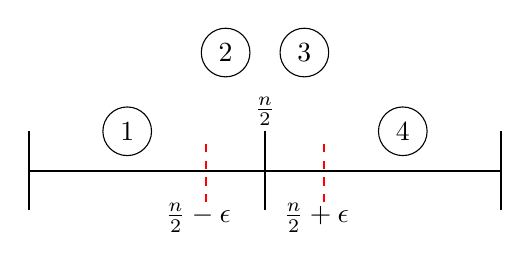
\begin{tikzpicture}
\draw[thick] (0,0) -- (6,0);
\draw[thick] (0,-0.5) -- (0,0.5);
\draw[thick] (6,-0.5) -- (6,0.5);
\draw[thick] (3,-0.5) -- (3,0.5);
\draw[thick, red, dashed] (2.25,-0.4) -- (2.25,0.4);
\draw[thick, red, dashed] (3.75,-0.4) -- (3.75,0.4);
\node (Ex) at (3,.75) {$\frac{n}{2}$};
\node (Ex1) at (2.15,-0.6) {$\frac{n}{2} - \epsilon$};
\node (Ex2) at (3.65,-0.6) {$\frac{n}{2} + \epsilon$};
\node[draw,circle] (1) at (1.25,.5) {1};
\node[draw,circle] (4) at (4.75,.5) {4};
\node[draw,circle] (2) at (2.5,1.5) {2};
\node[draw,circle] (3) at (3.5,1.5) {3};
\end{tikzpicture}
\end{center}
\begin{align}
\intertext{The distribution of numbers can be broken up into 4 segments. To get the median by the rank, it needs to be such that most of the numbers that are chosen are in sections 2 or 3. However, there is a problem that occurs when more than $\frac{t}{2}$ terms are in 1 or 4. As stated in the problem, we want}
\abs{r - \frac{n}{2}} &\leq \epsilon\frac{n}{2}\\
\frac{n}{2}-\epsilon\frac{n}{2} &\leq r \leq \frac{n}{2} + \epsilon\frac{n}{2}\\
\intertext{Which comes about from removing the absolute value sign. The probability that the element is in reagion 1 is the following}
P(\text{rank}(i)\in 1) &= \frac{\frac{n}{2}+\epsilon\frac{n}{2}}{n} = \left(\frac{1}{2}-\frac{\epsilon}{2}\right)\\
\intertext{This is the probability for one element to be found in region 1. What is needed is for more than $\frac{t}{2}$ to be in region 1}
\xi  &= \text{rank}(i)\in 1\nonumber\\
P\P{\xi \geq \frac{t}{2}} &= \P{\frac{1}{2} - \frac{\epsilon}{2}}^{\frac{t}{2}} + \P{\frac{1}{2} - \frac{\epsilon}{2}}^{\frac{t}{2}+1} + \cdots + \P{\frac{1}{2} - \frac{\epsilon}{2}}^{t}\\
P\P{\xi \geq \frac{t}{2}} &= \P{\frac{1}{2}-\frac{\epsilon}{2}}^{t}\left[ \sum_{i=0}^{\frac{t}{2}}   \P{\frac{1}{2}-\frac{\epsilon}{2}}^{i}\right] \\
 &= \P{\frac{1}{2}-\frac{\epsilon}{2}}^{\frac{t}{2}} \left[\frac{1-\P{\frac{1}{2}-\frac{\epsilon}{2}}^{\frac{t}{2}+1}}{1-\P{\frac{1}{2}-\frac{\epsilon}{2}}}\right]\label{Eq:Prob}\\
\intertext{Which is the probability of more than $\frac{t}{2}$ elements being in region 1. $\delta$ can be calculated from this. By revisiting the definition of probability in the question}
&P\P{\abs{r-\frac{n}{2}} < \epsilon\frac{n}{2}} \leq 1-\delta\\
&\delta = 1 - P\P{\abs{r-\frac{n}{2}} < \epsilon\frac{n}{2}}\\
&\delta = P\P{\abs{r-\frac{n}{2}} \geq \epsilon\frac{n}{2}}\\
\intertext{But what is wanted is the value in regions 1 and 4, and since they're symmetric it can just be multiplied by 2, giving}
&\delta = 2P\P{\abs{r-\frac{n}{2}} \geq \epsilon\frac{n}{2}}\\
\intertext{Using relation in Equation (\ref{Eq:Prob}) and plugging it in, we get}
&\delta = 2\cdot \P{\frac{1}{2}-\frac{\epsilon}{2}}^{\frac{t}{2}} \left[\frac{1-\P{\frac{1}{2}-\frac{\epsilon}{2}}^{\frac{t}{2}+1}}{1-\P{\frac{1}{2}-\frac{\epsilon}{2}}}\right]\\
\intertext{Now, for solving for $t$}
\xi &= \P{\frac{1}{2}-\frac{\epsilon}{2}}\\
\delta &= 2\xi^{\frac{t}{2}}\left[ \frac{1-\xi^{\frac{t}{2}+1}}{1-\xi}\right]\\
\underbrace{\frac{\delta}{2}\P{1-\xi}}_{\Omega} &= \xi^{\frac{t}{2}}-\xi^{t+1}\\
\intertext{Using Mathematica to solve this}
t &= \frac{2\log\left[\frac{\xi\sqrt{\frac{4\Omega\xi+1}{\xi^{2}}}-1}{2\xi}\right]}{\log(\xi)}
\end{align}
\end{solution}


\titledquestion{Amplification}

  Consider a decision problem $f$ (i.e one where the output is either zero or
  one). Suppose we are given a randomized algorithm $A$ that on input $x$ has
  the following properties:
  \begin{itemize}
  \item If $f(x) = 0$, then $A(x) = 0$
  \item If $f(x) = 1$, then $A(x) = 1$ with probability at least $2/3$.
  \end{itemize}
  Such an algorithm is said to have \emph{one-sided error}, and as we've
  discussed in class we can amplify the probability of being correct merely by
  repeating it a number of times, and returning $1$ if we ever see a $1$,
  returning $0$ otherwise.

  But suppose our algorithm instead had the following properties:
  \begin{itemize}
  \item If $f(x) = 0$, then $A(x) = 0$ with probability at least $2/3$
  \item If $f(x) = 1$, then $A(x) = 1$ with probability at least $2/3$.
  \end{itemize}
  In other words, it has \emph{two-sided} error rather than one-sided error.
  \begin{parts}
    \part[5] What is the probability of success (in either case) if we implement
    the above procedure (returning a $1$ if we ever see a $1$, else returning a
    zero) after $k$ iterations?
    \begin{solution}
      \begin{align}
        \intertext{The probability of success ($S$) is defined as}
        P(Success) &= P(S\cap f=0) + P(S\cap f=1)\\
                   &= P(S|f=0)\cdot \underbrace{P(f=0)}_{Assume\ \frac{1}{2}} + P(S|f=1)\cdot \underbrace{P(f=1)}_{Assume\ \frac{1}{2}}\\
        \intertext{The probability of getting all 0 for $f=0$ is $\left(\frac{2}{3}\right)^{k}$, while the probability of getting all 1 for $f=1$ is 1 minus the probability of getting all zero's for $f=1$, ie $\left(1-\frac{1}{3^{k}}\right)$}
        &= \P{\frac{2}{3}}^{k}\cdot \frac{1}{2} + \frac{1}{2}\cdot\P{1-\frac{1}{3^{k}}}
      \end{align}
    \end{solution}
\newpage
    \part[5] What is the probability of success (in either case) of the
    following procedure: Run the algorithm $k$ times and return the majority
    answer.
  \begin{solution}
  \begin{align}
    P\P{X_{0}>\frac{k}{2}} &\geq \sum_{i=1}^{\frac{k}{2}}\P{\frac{2}{3}}^{\frac{k}{2}+i}\P{\frac{1}{3}}^{\frac{k}{2}-i}\\
    &\geq \sum_{i=1}^{\frac{k}{2}}\frac{2^{\frac{k}{2}+i}}{3^{k}}\\
    &\geq \frac{1}{3^{k}}\sum_{i=1}^{\frac{k}{2}}2^{\frac{k}{2}+i} = \frac{1}{3^{k}}\left[ 2^{\frac{k}{2}+1}\right]\left[ 2^{\frac{k}{2}}-1\right]
  \end{align}
  \end{solution}
  \end{parts}

\titledquestion{The ``median'' trick}

Suppose we have an algorithm that generates independent samples $X_1,
\ldots$ of a random variable $X$. A natural estimate of the value of $X$ is the
mean $S = \sum_{i=1}^t X_i/t$ for some value of $t$. What is the probability
that $S$ is close to $\Exval{X}$? Specifically, what is the probability that $|S -
\Exval{X}| \le \epsilon \Exval{X}$? 

We can analyze this if we know that $\Var{X}$ is bounded. In particular, set $r
= \sqrt{\Var{X}}/\Exval{X}$. 

\begin{parts}
  \part[5] Show that if we set $t = O(r^2/\epsilon^2\delta)$ then the
  probability is at least $1-\delta$ (or in other words the probability of the
  difference \emph{exceeding} $\epsilon \Exval{X}$ is at most $\delta$). 
  \begin{solution}
    The figure below shows how the range of values can be partitioned. The values in parenthesis over each region is the probability of being in that region, which is what we're trying to prove.
\begin{center}
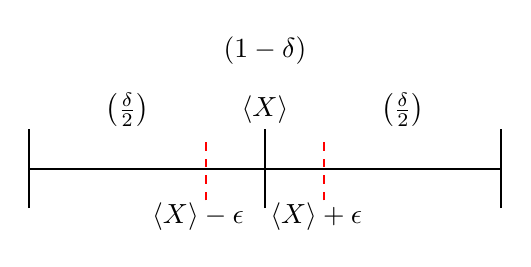
\begin{tikzpicture}
\draw[thick] (0,0) -- (6,0);
\draw[thick] (0,-0.5) -- (0,0.5);
\draw[thick] (6,-0.5) -- (6,0.5);
\draw[thick] (3,-0.5) -- (3,0.5);
\draw[thick, red, dashed] (2.25,-0.4) -- (2.25,0.4);
\draw[thick, red, dashed] (3.75,-0.4) -- (3.75,0.4);
\node (Ex) at (3,.75) {$\Exval{X}$};
\node (Ex1) at (2.15,-0.6) {$\Exval{X} - \epsilon$};
\node (Ex2) at (3.65,-0.6) {$\Exval{X} + \epsilon$};
\node (P1) at (1.25,.75) {$\left(\frac{\delta}{2}\right)$};
\node (P2) at (3,1.5) {$(1-\delta)$};
\node (P3) at (4.75,.75) {$\left(\frac{\delta}{2}\right)$};
\end{tikzpicture}
\end{center}
  \begin{align}
    \intertext{For simplicity, set the range to be the following variable}
    \alpha &= \Exval{X} - \epsilon\Exval{X} < \Exval{X} < \Exval{X} + \epsilon\Exval{X}\\
    \intertext{For the median to be outside $\alpha$, at least one has to be outside $\alpha$. The probability of choosing one outside of $\alpha$ is the following. From the defintion we have}
    P\P{\abs{X-\Exval{X}}\geq a} &\leq \frac{\Var{X}}{a^{2}}\\
    \intertext{Plugging in the relevant info}
    P\P{\abs{X-\Exval{X}}\geq \epsilon\Exval{X}} &\geq \frac{\Var{X}}{\epsilon^{2}\Exval{X}^{2}}\\
    \intertext{Which is the probability that it is not in the range. However, we have a set $t$, so the probability of one value of $t$ not being in the range is, and by plugging in $t=\BigO{\frac{r^{2}}{\epsilon^{2}\delta}}$}
    P\P{\abs{X-\Exval{X}}\geq \epsilon\Exval{X}} &\geq \frac{1}{t}\cdot\frac{\Var{X}}{\epsilon^{2}\Exval{X}^{2}} = \delta\ \checkmark
  \end{align}
  \end{solution}
\part[2] Suppose we only want a \emph{weak estimate}: an estimate $\tilde{X}$
that is within $\epsilon \Exval{X}$  with probability $2/3$. Show that in this case
we need only set $t = O(r^2/\epsilon^2)$. 
  \begin{solution}
  \begin{align}
    \delta &=1-\frac{2}{3}=\frac{1}{3}\\
    \frac{1}{3} &= \frac{1}{t}\cdot\frac{\Var{X}}{\epsilon^{2}\Exval{X}^{2}}\\
    &\Rightarrow t = 3\frac{r^{2}}{\epsilon^{2}} = \BigO{\frac{r^{2}}{\epsilon^{2}}}\ \checkmark
  \end{align}
  \end{solution}
\part[8] Now take the \emph{median} of $O(\log(1/\delta))$ such weak
estimates. Prove that this estimator does have the desired property of being
within $\epsilon \Exval{X}$ of the true estimate with probability $1-\delta$. Note
that we have done two things. 
\begin{enumerate}
\item We've reduced the number of samples needed from $r^2/\epsilon^2\delta$ to
  $r^2\log(1/\delta)/\epsilon^2$, which is an exponential reduction in
  dependence on $1/\delta$. 
\item We've achieved a strong bound without using full Chernoff-like
  assumptions: we only needed $X$ to have bounded variance. 
\end{enumerate}
  \begin{solution}
  \begin{align}
    \intertext{The median is represented in the above figure by $\Exval{X}$ such that there are bounds $\Exval{X}+\epsilon\Exval{X}$ and $\Exval{X}-\epsilon\Exval{X}$ for how accurate we want our {\em weak estimates} to be. If it doesn't lie in the interval, then at least half of them lie outside the interval with probability $\left(\frac{1}{3}\right)^{\frac{t}{2}}$. The probability needs to be less than $\delta$, so the upper bound on $t$ can be calculated by}
    \left(\frac{1}{3}\right)^{\frac{t}{2}} &= \delta\\
    3^{-\frac{t}{2}} &= \delta\\
    t &= 2\log\P{\frac{1}{\delta}} = \BigO{\log\P{\frac{1}{\delta}}}\ \checkmark
  \end{align}
  \end{solution}
\end{parts}
\newpage
\titledquestion{Hashing with open addressing}
We've seen how to use random hash function to ensure only a small number of
collisions in a hash bucket. We stored the overflow items in a \emph{chain},
which is why we wanted to minimize its length. Such a hashing scheme is called
\emph{chaining}. 

An alternate approach to hashing is called \emph{open addressing}. Suppose we
want to store $n$ items in an array. We maintain an array of $2n$ slots, and
also construct a hash function $h : U \times {\mathbb Z} \rightarrow [1\ldots
2n]$. For each key $k$, the sequence $h(k, 0), h(k, 1), \ldots$ defines a
\emph{probe sequence} as follows. 

\begin{itemize}
\item When $k$ appear, the algorithm first tries to place it in $h(k,0)$. If
  that entry is full, it tries $h(k, 1)$. If that is full, it tries $h(k, 2)$
  and so on.

\item   When searching for an item $q$, we search the entries
  $h(q, i), i = 0, 1, \ldots$ until we either find $q$ or find an empty spot
  (which means that $q$ was never in the set).
\end{itemize}

Assume that $h(k, j)$ is uniform over $[1\ldots 2n]$ for any $k$ and that all
$h(k, i)$ are independent. 

\begin{parts}
  \part[5] Show that the probability an insertion takes more than $r$ steps is
  at most $2^{-r}$. 
  \begin{solution}
  \begin{align}
    P(\text{collision}) &= \frac{1}{2n}\\
    P(\text{collision after filling $r$ buckets}) &= \P{\frac{1}{2n}}^{r}\\
    P(\text{collision after filling $r+1$ buckets}) &= \P{\frac{1}{2n}}^{r+1}\\
    P(\text{collision after $>r$ filled}) &= \sum_{i=r}^{n}\P{\frac{1}{2n}}^{i}\\ 
    &= \sum_{i=o}^{n-r}\P{\frac{1}{2n}}^{i+r} = \underbrace{\P{\frac{1}{2n}}^{r}}_{< 2^{-r}}  \underbrace{\left[ \frac{1-\P{\frac{1}{2n}}^{(n-r+1)}}{1-\P{\frac{1}{2n}}}\right]}_{<1}\\
    &\therefore P(\text{collision after $> r$ filled}) < 2^{-r}\ \checkmark
  \end{align}
  \end{solution}
\part[5] Show that for the $i^{\text{th}}$ insertion ($i = 1, 2, \ldots, n)$, the
  probability that more than $2\log n$ probes are needed is $1/n^2$. 
  \begin{solution}
  \begin{align}
    \intertext{Simply set $r$ to $2\log (n)$}
    2^{-2\log(n)} = \frac{1}{n^{2}}
  \end{align}
  \end{solution}
\newpage
\part[5] Let $X_i$ be the number of probes needed to insert item $i$, and let $X
= \max X_i$. Show that $\Pr(X > 2 \log n) \le 1/n$. 
  \begin{solution}
  \begin{align}
    \intertext{From the question, we know that we can set $X$ to be the following}
    X &= \max{X_{i}}\\
    \intertext{This leads to $n$ different probabilities in it, but since it's the maximum $X$ (which is $n$) then they are all the same probabilities, and you simply sum over all $n$ of them}
    \sum_{i=1}^{n}P(X > 2\log(n)) &= P(X > 2\log(n)) + P(X > 2\log(n)) + \cdots + P(X > 2\log(n))\\
    &= n\cdot P(X > 2\log(n)) = n\cdot\frac{1}{n^{2}} = \frac{1}{n}\ \checkmark
  \end{align}
  \end{solution}

\end{parts}

\titledquestion{Derandomizing MAX CUT}

While randomness is an easy way to design an algorithm, random bits are an
expensive resource, and we'd like to use as few of them as possible. The process
of removing randomness from an algorithm is called \emph{derandomization}. There
are three basic approaches to derandomization: using weak randomness,
eliminating randomess by brute force, and the method of conditional
expectations. We will examine the latter two methods here. 
\begin{parts}
  \part[5] Suppose we have a randomized algorithm that runs in time $T(n)$, 
  uses $O(\log n)$ random bits and returns the minimum of some function with a
  probability of success greater than $2/3$.  Construct a deterministic algorithm that solves
  the same problem correctly in time $T'(n)$, expressed in terms of $T(n)$ and $n$
  (\textbf{Hint:} this is called the method of brute force). 

  The other approach works as follows. Suppose our randomized algorithm $A$ produces
  some answer whose expectation is $\mu$. We can imagine the algorithm as a
  sequence of deterministic operations punctuated by coin tosses $r_1, r_2,
  \ldots, r_m$. The value output by $A$ is a function of the input and these
  coin tosses: ignoring the input, we can write the output value as $A(r_1,
  \ldots, r_m)$, and so $E[A(r_1, \ldots, r_m)] = \mu$

  Consider the first coin toss $r_1$. We can write 
\[ E[A(r_1, \ldots, r_m)] = (1/2)E[A(0, r_2, \ldots, r_m)] + (1/2)E[A(1, r_2,
\ldots, r_m)] \]
This is because the probability of $r_1 = 1$ is $1/2$. Notice however that one
of the two expectations $E_0 = E[A(0, r_2, \ldots, r_m)]$ and $E_1 = E[A(1, r_2,
\ldots, r_m)]$ must be at least as large as $\mu$ (since $\mu = (E_0 +
E_1)/2$). Suppose we can compute these two numbers. Then we can
\emph{deterministically} pick the value of $r_1$ and we are sure that the final
answer we get is no worse than the expected value, while having used one less
random bit. 

Repeating this over and over again yields a final result in which all bits are
picked deterministically, and yet the final answer is at least as large as
$\mu$. Thus, we've derandomized the algorithm without paying a penalty. The catch is of course the estimation of $E_0$ and $E_1$. 

Now consider the randomized algorithm for MAX CUT that yields a
$0.5$-approximation: Pick a vertex and label it as being black or white with
equal probability. Repeat for all vertices, and return the partition into black
and white as the desired cut. 

  \begin{solution}
    For a randomized algorithm, it takes in values such as \verb~RA(X,r)~ where \verb~X~ is some input and \verb~r~ is some random value. This can be turned into a deterministic algorithm \verb~DA(X)~ by the following algorithm
    \begin{algorithmic}
    \FOR{$i=1$ \TO $n$} \STATE{\IF{\verb~RA(X,~$i$\verb~)~ $<$ \verb~min~} \STATE{$\verb~min~=\verb~RA(X,~ i \verb~)~$} \ENDIF} \ENDFOR
    \RETURN{\verb~min~}
    \end{algorithmic}
  This yields a time complexity for the deterministic algorithm of 
\[
T^{\prime}(n) = p(n)\cdot T(n)
\]

Where $p(n)$ is some polynomial at least $\BigO{n}$
  \end{solution}

\part[10] Derandomize this algorithm using the method of conditional
expectations. What is the resulting deterministic algorithm? (\textbf{Hint:}
think about how we might deterministically decide which color to give to a
vertex based on the graph structure and how it influences $E_0, E_1$.)
  \begin{solution}
    An algorithm for deterministic coloring based off of the graph structure is:
    \begin{enumerate}
      \item Find the node with the highest degree. If there are multiple values, then choose one of them at random.
       \item Color the given node one color, and color all the adjacent nodes the opposite color.
         \begin{itemize}
           \item {\em For Example:} Color the highest degree vertex black and all connecting verticies white.
         \end{itemize}
      \item Find the highest degree that is not-colored and go back to step 2.
    \end{enumerate}
The analog to this in the max-cut problem is deleting all of the edges at those 
who are black, and leaving for all the white edges. Doing this will give the 
edges that need to be removed from the graph and give the Max Cut.
  \end{solution}
\end{parts}

\end{questions}
\end{document}
